%!TEX root = ../Security&NetworkManagement.tex
\chapter{Introduzione}
Il concetto di \textit{sicurezza} (\textit{security}) può essere brevemente descritto come la protezione delle informazioni di un sistema da furti o dal danneggiamento hardware o software del sistema stesso. Le principali proprietà della sicurezza sono tre:
\begin{itemize}
	\item \textbf{Confidenzialità}. Garantire che l'informazione non sia accessibile da persone non autorizzate.
	\item \textbf{Integrità}. Garantire che l'informazione non sia alterata da persone non autorizzate in un modo che non è rilevabile dagli utenti autorizzati.
	\item \textbf{Autenticazione}. Assicurare che gli utenti siano le persone che dicono di essere.
\end{itemize}
Raggiungere questi obiettivi, tuttavia, non è così semplice.\\
È molto comune, inoltre, confondere il concetto di \textit{security} con quello di \textit{safety}:
\begin{itemize}
	\item \textbf{Security}. Con questo termine si esprime l’insieme delle misure finalizzate a \textit{prevenire} o \textit{ridurre} la probabilità che un dato evento non desiderato accada.
	\item \textbf{Safety}. Con questo termine si intende invece la \textquotedblleft risposta" del sistema al verificarsi di un particolare evento indesiderato. La safety è legata a pericoli/danni a persone, e non solo a cose.
\end{itemize}
In generale si cerca security per la safety di un sistema (e.g. torre di controllo in un aeroporto). Inoltre, è sempre bene tenere presenti i \textit{costi} legati alla sicurezza: la sicurezza non è gratuita. Questa infatti implica una complessità maggiore del sistema, maggiori costi operazionali e di implementazione ed il cambiamento del workflow (alcune cose potrebbero non essere fattibili, o potrebbero essere realizzate con limitazioni).

Prima di progettare la parte riguardante la sicurezza di un sistema, abbiamo bisogno di conoscere \textit{che cosa} (\textit{what}) deve essere reso sicuro, \textit{perché} (\textit{why}), e \textit{contro chi} (\textit{who}). Quando le politiche di sicurezza sono troppo restrittive (o non sono comprese) l'utente troverà un modo per violarle; d'altra parte, le politiche di sicurezza, se non seguite, risultano \textit{inutili}.

Il problema diventa quindi il seguente: abbiamo bisogno di un modo per descrivere \textit{che cosa, perché} e \textit{contro chi}. Per questa necessità in genere si segue uno standard, l'\textbf{Enterprise Architecture Framework (EAF)}.

\section{Enterprise Architecture Framework}
Un \textit{Enterprise Architecture Framework (EAF)} (Figura \ref{img:EAF}(a)) è un framework per un'architettura d'impresa; in particolare, definisce come organizzare la struttura, le viste associate con un'architettura d'impresa, gli scopi e tutte le sotto-strutture fino alle unità semplici. Sostanzialmente è qualcosa legato alla gestione dell'azienda ed abbiamo bisogno di comprenderlo per utilizzarlo.
\begin{figure}[htbp]
	\centering
	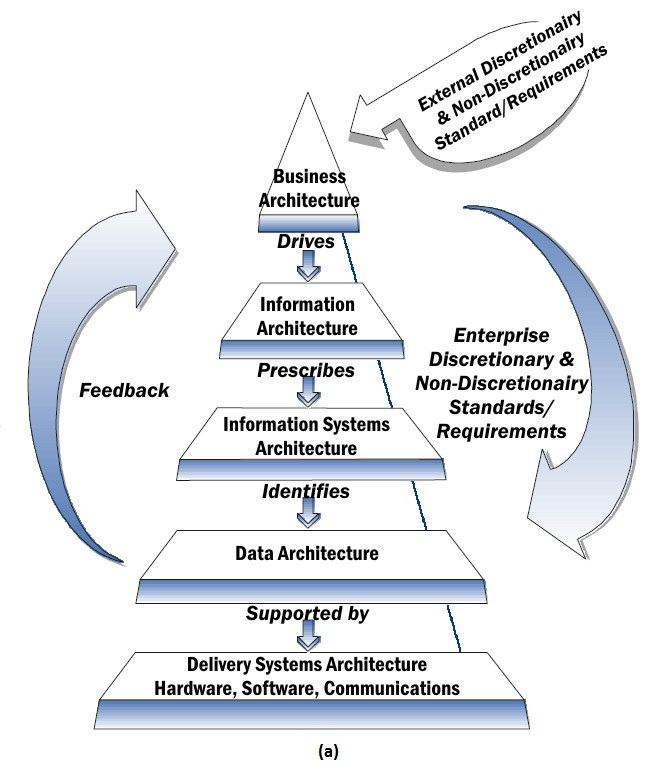
\includegraphics[scale = 0.4]{images/EAF_scheme.jpg}\qquad\qquad
	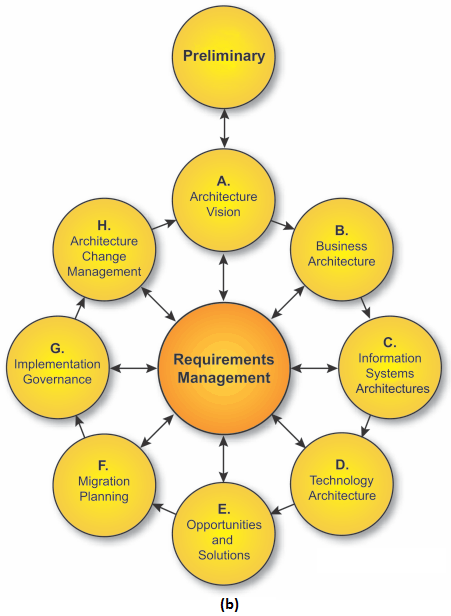
\includegraphics[scale = 0.5]{images/EAF_iterative_model}
	\caption{Enterprise Architecture Framework.}
	\label{img:EAF}
\end{figure}
Gli EAFs più usati sono i seguenti:
\begin{itemize}
	\item COBIT -- Framework for IT Governance and Control
	\item TOGAF -- The Open Group Architecture Framework
	\item DoDAF -- United States Department of Defense Architectural Framework
	\item MODAF -- United Kingdom Ministry of Defence Architectural Framework
	\item NAF -- the NATO Architecture Framework
	\item SABSA a comprehensive framework for Enterprise Security Architecture and Service Management
\end{itemize}
TOGAF e COBIT sono quelli più usati in imprese non militari. In Figura \ref{img:EAF}(b) è riportato l'EAF TOGAF: questo, come altri EAFs, adotta un modello \textquotedblleft iterativo" in cui ad ogni fase si raffinano e si precisano i concetti precedenti. Gli aspetti ingegneristici/tecnici sono racchiusi principalmente nei punti F, G e H. Gli EAF moderni hanno una struttura circolare:
\begin{itemize}
	\item Passo 0. Preliminari. Statements che descrivono l'azienda.
	\item Passo A. Dal primo passo si creano le Architecture Vision (ovvero il \textit{come} è strutturata l'azienda)
	\item Passo C. Information System: che cosa ho bisogno di sapere? Quali informazioni? Quali limiti?
	\item Passo D. Tecnology Architecture, devo riuscire a fare l'information e l'architecture (Problema dei Requisiti)
\end{itemize}
Gli altri passi implicano la gestione, la manutenzione e l'implementazione dell'architettura. Lo schema è molto simile alla programmazione agile (Modello a V). Dopo il passo D si dovrebbe avere un sistema funzionante; le fasi successive servono per dare vita all'azienda. Gli EAF producono dei documenti standard che descrivono cosa viene fatto in ogni fase. Si noti che ogni step produce uno o più requirements che il concetto dopo deve risolvere, altrimenti si ritorna indietro. Quasi tutti i framework pongono l'accento sui dati piuttosto che sulle applicazioni o sulla tecnologia. A tal proposito viene introdotto il concetto di \textit{asset}, definito nel passo A.

Si definisce \textbf{asset} una qualsiasi risorsa dell'impresa che abbia o rappresenti un valore importante per l'azienda stessa; può essere rappresentato da: dati, componenti tecnologici (hardware) o componenti applicativi (applicazioni).\\
Per garantire la sicurezza su un asset è necessario che tutta la catena dell'EAF corrispondente sia implementata in maniera affidabile. Un asset ha anche delle proprietà che possono essere intrinseche, desiderate o imposte dalla legge (e.g. i dati personali sono sottoposti alla legge sulla privacy). Tali proprietà sono \textquotedblleft esportate" agli asset che interagiscono con l'asset in questione. Lo scopo principale della sicurezza è quello di proteggere gli asset. Gli assets sono di due tipi:
\begin{itemize}
	\item \textbf{Primario}. Se compromessi, l'azienda si ferma o subisce gravi danni.
	\item \textbf{Secondario}. Se compromessi, il danno è minimale o nullo.
\end{itemize}
La sicurezza degli assets non viene aumentata in modo casuale, bensì rispettando dei requirements. I vari assets devono interagire tra loro a seconda delle loro proprietà. Gli assets vengono decisi dall'azienda e dalla legge. È molto importante capire bene i requirements dell'asset al fine di svolgere un'analisi quanto più dettagliata possibile. Introduciamo dunque il \textit{risk management}.\\
La gestione del rischio (\textbf{risk management}) è il processo mediante il quale si misura o si stima il rischio (in riferimento agli asset) e successivamente si sviluppano delle strategie per gestirlo. Il risk management è diverso dall'enforce management, poiché siamo consapevoli che un qualche tipo di rischio esiste sempre. La gestione dei rischi è molto complicata, perché per gestire un rischio è necessario in primis \textit{identificare tutti i tipi di rischi possibili} di un asset; in secondo luogo vi è una fase di \textit{valutazione} in cui si decide se il rischio è reale o meno, ossia se tale rischio ha una probabilità ragionevole di verificarsi, e quanto può essere dannoso per sistema. Solo dopo questi due passi è possibile pensare alle tecniche di \textit{riduzione del rischio a livelli accettabili} (si cerca di evitare il verificarsi di un evento dannoso) ed \textit{implementazione di contromisure per mantenere il livello di rischio definito}. Ciò che siamo abituati a pensare come “sicurezza” è svolto negli ultimi due punti. Ad esempio per un hard disk la riduzione del rischio si traduce nell'acquisto di uno migliore, mentre una contromisura è il backup.

Una volta terminata la parte di gestione del rischio, si procede con la valutazione del rischio (\textbf{risk assessment}). Esistono due tipi di risk assessment:
\begin{enumerate}
	\item \textbf{Qualitativo}. Fornisce una visione semplice e sintetica dei possibili rischi.
	Per svolgere un risk assessment di tipo qualitativo si utilizzano dei valori relativi (ad esempio una scala da 1 a 3, dove 1 significa \textquotedblleft low", 2 significa \textquotedblleft medium" e 3 significa \textquotedblleft high"). Questi valori producono un ordinamento dei rischi in base alla loro priorità che può essere utile durante il processo di risk management.\\
	Alcuni esempi di analisi qualitativa possono essere la costruzione di matrici di importanza (influenza) (una per ogni asset) o la stima della probabilità di occorrenza. Di seguito è riportato un esempio di matrice di importanza.
	\begin{center}
		\begin{tabular}{ c|c|c|c| }
			\cline{2-4}
			High &  &  & \\
			\cline{2-4}
			Med &  &  & \\
			\cline{2-4}
			Low &  &  & \\
			\cline{2-4}
				\multicolumn{1}{r}{} &  \multicolumn{1}{c}{Low}
			& \multicolumn{1}{c}{Med} & \multicolumn{1}{c}{High} \\
		\end{tabular}
	\end{center}
	Le righe (asse $y$) contengono la probabilità che un evento $e$ accada ($\mathcal{P}(e)\in\{\text{low, med, high}\}$), mentre le colonne (asse $x$) contengono il risultato (outcome) dell'evento. Una volta costruita la matrice, questa viene suddivisa in tre parti tracciando due diagonali; chiamiamo la parte più bassa $A$, quella nel mezzo $B$ e quella più in alto $C$. Dobbiamo quindi focalizzarci in primis sulla parte $C$ per cercare di portare quanto più possibile nella parte $B$: questo può essere effettuato mediante la riduzione della probabilità del verificarsi di un evento o tramite la riduzione dell'outcome. Analizziamo poi la parte $A$ ed in questo caso abbiamo due possibilità:
	\begin{enumerate}
		\item I rischi identificati non sono correlati al lavoro.
		\item I rischi identificati sono correlati; in questo caso, o abbiamo sovrastimato l'evento o abbiamo speso troppo per la sicurezza.
	\end{enumerate}
	Vantaggi di un approccio qualitativo: semplice e di immediata comprensione per qualsiasi lettore. Svantaggi: serve un esperto del sistema per costruirlo, dunque per raggiungere la semplicità dobbiamo consultare un esperto che sappia nel dettaglio qualsiasi cosa inerente al sistema: se non realizzato da un esperto, questo modello potrebbe produrre dei risultati troppo approssimativi o incorretti.
	\item \textbf{Quantitativo}. In questo caso si parte da un insieme di formule matematiche, si assegna un'unità di misura ad ogni asset ed infine si associa un valore ad ogni asset (detto \textit{Asset Value -- AV}). Successivamente si calcola l'\textit{Annual Rate of Occurrence (ARO)}, ossia il numero di volte che ci aspettiamo che un evento accada in un anno, e l'\textit{Exposure Factor (EF)} [\%] che indica la percentuale di un asset che ci si aspetta di essere danneggiato da ogni occorrenza di un particolare rischio (e.g. se ci aspettiamo che un rischio distrugga completamente un asset, $EF=100\%$).\\
	Dati questi tre valori, si calcolano altri due valori derivati: la \textit{Single Loss Expectancy (SLE)} e l'\textit{Annual Loss Expectancy (ALE)}. La SLE indica il valore che ci aspettiamo di perdere ogni volta che un rischio si verifica: SLE $ = $ AV $\times$ EF. L'ALE indica il valore medio che ci aspettiamo di perdere ogni anno per un dato rischio: ALE $ = $ SLE $\times$ ARO; in genere questo valore si utilizza per prendere decisioni riguardanti le misure che dovrebbero essere adottate per gestire i particolari rischi. Infatti, se l'ALE è alto è possibile:
	\begin{itemize}
		\item implementare delle contromisure per ridurre la probabilità del verificarsi dell'evento, oppure
		\item lavorare sull'EF, cercando di ridurre le conseguenze (cioè di ridurre l'outcome nel modello precedente).
	\end{itemize}
	Questo modello tuttavia presenta alcune criticità:
	\begin{itemize}
		\item non è semplice quantificare il valore di un asset;
		\item l'ARO è una probabilità che non è semplice da stimare;
		\item non è semplice valutare l'EF.
	\end{itemize}
	Il prodotto di questi ultimi tre valori fornisce l'ALE, in cui l'errore è amplificato dal momento che anche gli errori di stima di ogni singolo fattore sono moltiplicati. Se quindi non vi è una sufficiente accuratezza nella stima di questi tre parametri otteniamo delle misure troppo grossolane. Come ultima cosa si tenga presente che l'ALE è un valore medio, dunque per avere più precisione nella stima tipicamente viene utilizzata la moda (il valore più alto nella distribuzione).
\end{enumerate}
A questo punto entra in gioco la \textbf{risk analysis} (che indica cosa produce il rischio sull'asset) che presentiamo mediante il modello grafico (Figura \ref{img:risk_analysis_model}); descriviamolo brevemente. 
\begin{figure}[htbp]
	\centering
	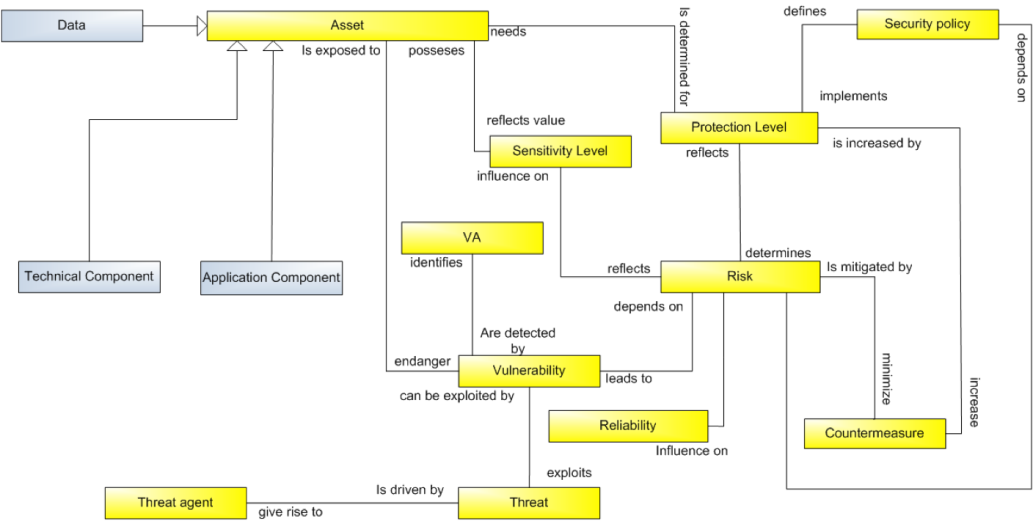
\includegraphics[scale = 0.4]{images/risk_analysis_model}
	\caption{Risk Analysis Model.}
	\label{img:risk_analysis_model}
\end{figure}

Un \textit{asset} ha due proprietà: il \textit{livello di sensitività}, cioè quanto un asset è sensibile ad un rischio (e dunque riflette la proprietà di sicurezza che vogliamo attribuire all'asset), ed il \textit{livello di protezione}, cioè il livello di sicurezza che diamo all'asset. La seconda proprietà definisce le \textit{security policies}, delle misure preventive per far sì che un dato evento non accada (costose in generale), ed implementa delle \textit{contromisure} atte a ripristinare gli effetti negativi causati dal verificarsi di un evento. Il livello di protezione riflette i rischi, che sono influenzati da \textit{reliability} e \textit{vulnerability}. La reliability non dipende dall'asset, ma da \textquotedblleft qualcosa di fisico". La vulnerability è un aspetto che viene spesso sfruttato in rete dagli attaccanti ed è una proprietà degli asset (ossia l'asset è vulnerabile); in sostanza la presenza di vulnerabilità implica la presenza di pericoli per il sistema, in particolare per l'asset stesso. Un \textit{threat}, ideato da un \textit{threat agent}, sfrutta le vulnerabilità per attaccare un asset. Si noti che la vulnerabilità, in generale, non è nota a priori da un attaccante: essa deve essere prima trovata e qualora lo fosse, questa rappresenta un pericolo per l'asset. La vulnerabilità va dunque \textit{eliminata} e non nascosta: principalmente le vulnerabilità devono essere eliminate mediante una buona progettazione/programmazione dei sistemi. Una parte chiave in questo processo è quindi il \textbf{vulnerability assessment} che può essere attuato in diversi modi. Si noti che nessun programma è bug-free: le vulnerabilità esistono sempre.

Per definire in modo completo la “sicurezza” è infine indispensabile il \textbf{threat model} (attaccante), descritto nell'RFC 3552, che fa parte della risk analysis. Come già detto, un asset ha sicuramente delle vulnerabilità, e queste possono essere note oppure completamente ignote all'attaccante. In ogni caso è necessario costruire un modello che ci indichi quanto potenti sono le risorse ed informazioni che possiede un attaccante. Il threat model si pone di descrivere principalmente tre questioni: le \textit{informazioni} che possiede l'attaccante sul sistema, la \textit{capacità computazionale} dell'attaccante e “quanto” sta \textit{controllando il nostro sistema}. Generalmente si assume che l'attaccante abbia a disposizione tutte le informazioni del sistema (tranne le chiavi di crittografia), abbia un'ottima dotazione HW/SW, abbia un totale controllo del sistema di comunicazioni (send/receive), ma si suppone che l'attaccante non abbia ancora preso controllo degli endpoints (sistema).

In alcuni casi è plausibile parlare di attacchi “limitati”, dove l'attaccante può alternativamente:
\begin{itemize}
	\item inviare ma non ricevere [tutto] (\textbf{attacchi attivi}, bind o meno); con questo tipo di attacco si mandano dei pacchetti in rete, ma potrebbe essere persa di vista la comunicazione tra gli endpoints. Alcuni esempi sono: replay attacks, message insertion (aggiunta di contenuto nei messaggi), message deletion, message modification e man-in-the-middle (l'attaccante si pone nel canale di comunicazione tra endpoints svolgendo così il ruolo di proxy, ma allo stesso tempo può manipolare i messaggi a suo piacimento).
	\item ricevere ma non inviare (\textbf{attacchi passivi}). Questo è un tipo di attacco difficile da fare senza essere notati: le reti switched, avendo capacità di trasmissione di $\approx$ 1Gb/s, eventuali flussi massicci di dati rallenterebbero sicuramente la velocità di trasmissione nella rete. Questo perché in genere vengono catturati \textit{tutti} i pacchetti che transitano da/verso uno o più host al fine effettuare alcune operazioni come violazione di confidenzialità, password sniffing oppure offline cryptographic analysis.
\end{itemize}
Un altro elemento sul quale bisogna porre l'attenzione è la topologia della rete. Ai fini della sicurezza è necessario conoscere sia la topologia fisica, sia quella IP. L'idea è quella di controllare il percorso delle informazioni per cercare di capire se queste passano per un attaccante. È assolutamente sbagliato assumere che l'attaccante possa inviare e ricevere pacchetti con la stessa facilità.\\
Gli attacchi si possono dividere in:
\begin{enumerate}
	\item \textbf{On-path}: l'attaccante si trova sul percorso dei pacchetti (e.g. man-in-the-middle). Di solito solo un gateway o un router sono on-path. Sono possibili solo attacchi attivi, ma non blind o passivi.
	\item \textbf{Off-path}: è il caso normale (passivo, cioè di tipo blind). L'attaccante può non trovarsi sul percorso delle informazioni. Sono attacchi al routing e alla capacità di rete. È possibile effettuare solo attacchi attivi blind, perché non è possibile sentire i pacchetti tra $A$ e $B$ del path.
	\item \textbf{Link-local}: sono gli attacchi peggiori, l'attaccante è sulla stessa sottorete di uno degli endpoints.
\end{enumerate}
Non si deve mai assumere che l'attacco sia off-path, ma certamente è più difficile (e meno probabile) che sia on-path. Inoltre per “diventare” on-path è necessario portare un attacco alla topologia (routing); questo è possibile ma assolutamente non banale.\\
Ricapitolando, un attacco:
\begin{enumerate}
	\item non è mai fine a sé stessi, vi è sempre uno scopo. È sempre necessario chiedersi il \textit{perché}.
	\item sfrutta una vulnerabilità.
	\item è rivolto ad un \textit{asset}.
\end{enumerate}
Un asset, invece:
\begin{enumerate}
	\item presenta \textit{sempre} delle vulnerabilità.
	\item ha un protection level ed un sensitivity level.
	\item si può proteggere con delle \textit{contromisure}.
\end{enumerate}
Le contromisure non sono le protezioni contro le vulnerabilità (queste ultime infatti sono tese ad eliminare le vulnerabilità). Le contromisure possono essere viste come vie alternative nel caso in cui l'asset venga attaccato.